\subsection*{Designovervejelser og afgrænsning (Christian)}
\addcontentsline{toc}{subsection}{Designovervejelser og afgrænsning}
Udfra kravspecifikationen og analysen lagde vi os fast på vores design valg. Da
vores system skal køre på mange forskellige systemer (måske endda mobile
devices) og helst uden installation, valgte vi en web-baseret løsning. Dette gav
senere nogle udfordringer mht. GRASP patterns da servlet og web-side referencer
foregår som til en Singleton og det eneste objekt, der er garanteret at
persistere mens brugeren anvender systemet er session objektet - Hvert nyt
browser request behandles som en separat kørsel af et program og kun session
objektet bevares for hver bruger.\\
Da der skal være sporbarhed i systemet, bør data ikke kunne slettes i
databaserne. Ingen af vores DAO klasser skal således implementere en 'delete'
funktionalitet. Vores brugere skal dog kunne inaktiveres hvilket skal
reflekteres i databasen.\\
Det var ikke muligt for os at interface med cpr-register eller
hospitalsdatabaser, hvorfor vi ikke kunne hente patientdata fra et ekstent
system. For at imødekomme en eventuel fremtidig mulighed for interfacing med et
eksternt system uden for stor omskrivning af kodebasen, valgte vi at udskille
patientens data i et eget data transfer object, som ville kunne hentes via et
nyt data access object der forbinder til et eksternt system. Login
funktionalitet implementeres som en serverside cookie der holder styr på bruger
og privilegier.\\
For at minimere antallet af museklik og transaktioner, valgte vi at samle
rekvisitioner og kontrolskemaer i samme view. Vores frontend sørger for at
skjule kontrolskemaer der ikke er relevante for den aktuelle undersøgelse. På
den får vi også samlet ensartet funktionalitet for de forskellige kontrolskemaer
i den samme controller.\\
\FloatBarrier
\begin{figure}[h]
\subsection*{Pakke diagram (Morten)}
\addcontentsline{toc}{subsection}{Pakke diagram}
\centering
\makebox[\textwidth]{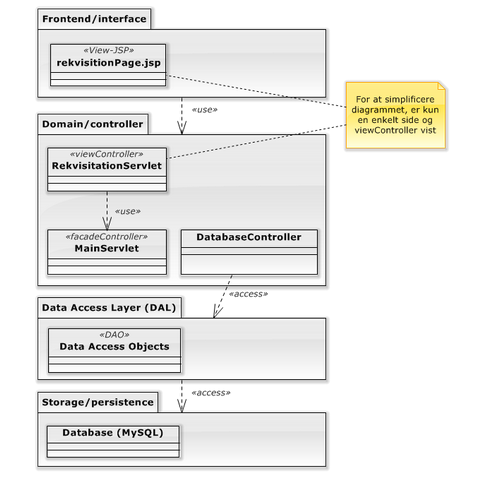
\includegraphics[width=\textwidth]{Pakke_diagram}}
\caption{\emph{Pakkediagram}. Viser en overordnet inddeling af programmet i lag
i model-view-controller - med en opdeling af modellaget i DAL lag og Persistence
lag. \label{pakke_diagram}}
\end{figure}
\FloatBarrier
\subsection*{Klassediagram (Rúni, Christian, Martin)}
\addcontentsline{toc}{subsection}{Klassediagram}
Udfra vores domænemodel og designovervejelser mappede vi til et
designklassediagram. Som nævnt giver webarkitekturen nogle udfordringer - også
med hensyn til modelleringen. Alle servlets og .jsp-sider tilgås via et browser
request, der kan opfattes som en start af et nyt seperat programinstans. Bag
vores system ligger Apache Tomcat serveren, der modtager browser requestet -
pakker det i et request object og linker et session objekt, der er specifikt for
den bruger, der tilgår vores domæne. Session objektet persisterer mellem hvert
af brugerens requests og vi bruger det derfor til at holde styr på objekter, der
skal bruges under hele brugerens session.\\
Serveren sender herefter requestet videre til den .jsp side eller servlet som
brugeren forsøger at tilgå. Serveren instantierer et instans\footnote{ Ved høj
load kan serveren sættes op til at instantiere mere end et instans.} af hver
Servlet klasse og giver referencen til instansen ud fra requestet - Servletsne
opfører sig således som en slags Singletons. Man kan altså på et hvilket som
helst tidspunkt tilgå en servlet eller .jsp side ved at indtaste deres adresse
og det er derfor ikke nødvendigt at gå gennem MainServlet for at tilgå de andre
servlets. Derfor er relationerne mellem Servlets og .jsp sider modeleret som use
relations.\\
Vi har i vores arkitektur alligevel forsøgt at holde low coupling. Vores views
(.jsp siderne) kender således kun deres egen controller og sender data videre
til dem når brugeren interagerer med siden. På samme måde kender vores view
controllers ikke hinanden, men tilgår hinanden gennem MainServlet instanset, der
videredelegerer ansvaret. På den måde opnår vi at vi kan udskifte controllers
uden at opdatere referencer andre steder end i MainServlet. Anvendte patterns er
i øvrigt beskrevet i detaljer i \hyperref[design_patterns]{Design Patterns
afsnittet}.
\FloatBarrier
\begin{figure}[h]
\centering
\makebox[\textwidth]{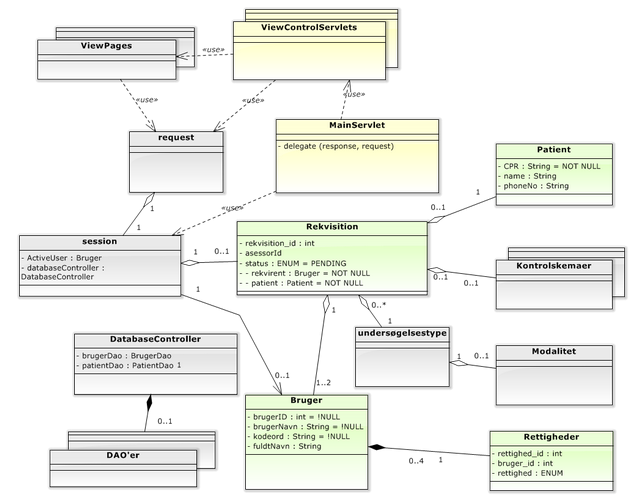
\includegraphics[width=\textwidth]{klasse_diagram}}
\caption{\emph{Klassediagram} over hele systemet. Controllers er markeret med
gul baggrundsfarve, DTO’er med grøn, JSP-sider med grå. \label{klasse_diagram}}
\end{figure}
\FloatBarrier
For overskuelighedens skyld er adskillige use relations udeladt - Alle servlets
tilgår eksempelvis session objektet og dets bruger for at kontrollere om
brugeren er logget ind. jsp siderne har formelt en use relation til deres eget
view, der også er udeladt. Et mere fuldstændigt diagram kan ses i
\hyperref[Bilag25]{bilag 25}.
\subsection*{Design Patterns (Christian, Rúni)}
\addcontentsline{toc}{subsection}{Design Patterns} \label{design_patterns}
Vi har forsøgt at implementere flere forskellige patterns for at honorere vores
non funktionelle krav til systemet.
\subsubsection*{GRASP\cite{larman}}
\addcontentsline{toc}{subsubsection}{GRASP}
\begin{itemize}
  \item \emph{Controller} - Events der ikke er brugergrænseflade relaterede
  bliver håndteret af en gruppe af controllers der formidler kontakten med vores
  model lag - på den måde overholder vi også Model View Controller patternet.
  Forrest har vi en facade controller der ikke selv interagerer med View eller
  Model, men videredelegerer ansvaret til vores use case-controllers. Use case
  controllers er tænkt til at håndtere handlinger der er relateret til en af
  vores main use cases. Vi bryder 2 steder med patternet - hhv. i frontenden,
  hvor inputvalidering foretages i javascript direkte i viewet. Dette gør
  serveren og internet forbindelsen ikke belastes af et kald til vores centrale
  system, hvilket giver en bedre performance. Ligeledes har vi valgt at
  implementere domæneregel “Over 18” på database niveau som en trigger, hvilket
  betyder at modellaget får controlleropgaver. På den måde undgår vi at omskrive
  vores javakode, når der tilkommer nye domæneregler - de kan i stedet
  implementeres som triggers/stored procedures på databaseniveau.
  \item \emph{Creator} - Vi har ikke fået opfyldt creator pattern, da
  oprettelse af et rekvisition objekt ikke selv opretter sine tilhørende objekter (Patient,
  Rekvirent, Kontrolskemaer og evt. Visitator), men de istedet skal oprettes i
  control laget, og derefter blive klistret på, dette ses for eksempel i
  “NyRekvisitionServlet”. Også hvis man skal gemme en rekvisition, kan
  rekvisition DAO’en ikke gemme de tilhørende objekter, og bliver det løst ved
  at controlleren skal have fat i de manglende DAO’er for at objekterne skal
  blive gemt. Dette er en oplagt fremtidig implementering.
  \item \emph{High Cohesion} - Vi har forsøgt at holde vores objekter
  fokuserede. Vores delelementer af systemet har således veldefinerede opgaver
  og kan således genbruges og erstattes uden store kodeændringer. Eksempelvis
  har vi tilføjet en databaseController mellem dao objekterne og session
  objektet, som laver en højere binding mellem session objektet og
  databaseControlleren og samtidig også en lavere kobling til session objektet.
  \item \emph{Information Expert} - I samme tråd er metoder og data relateret
  til et givent ansvars område søgt samlet i enkelte objekter. DAO'erne er
  eksempler på klasser, der håndterer det specifikke ansvarsområde at gemme og
  hente DAO'er.
  \item \emph{Indirection/Pure fabrication} - Vi havde i vores initielle løsning
  mange koblinger til sessionobjektet - herunder 11 DAO'er. For at reducere
  antallet af koblinger valgte vi at indskyde en ekstra controller,
  databaseController, der håndterer DAO'er, herunder oprettelse.
  DatabaseControlleren repræsenterer ikke noget objekt fra vores domænemodel, og
  er således også en 'pure fabrication'. I samme proces øges bindingen, da DAO
  relaterede opgaver samles i samme objekt, i stedet for at blandes med andre
  opgaver i sessionobjektet.
  \item \emph{Low Coupling} - Vi har opnået low coupling ved at arbejde med de
  ovenstående patterns. Da vores Servlets interagerer kun med sin “egen” jsp
  side og mainServletten, i stedet for at tilgå hinanden direkte, bliver
  koblingen meget lavere. Samme måde er anvendt, ved at lave en
  databaseController mellem session og DAO’erne, hvilket giver lavere kobling
  til session objektet.
  \item \emph{Polymorphism} - Vi beskytter os mod gentagen kode ved at anvende
  arv. Eksempelvis extender vores servlets HTTPServlet interfacet og den
  funktionalitet de deler er beskyttet i superklassen. Vores DAO'er extender
  AbstractDAOImpl, hvor funktionalitet der er fælles for vores DAO'er er samlet.
  Vores servlets kunne i højere grad anvende arv, da nogle metoder går igen -
  eksempelvis går metoden til at udsøge rekvisitioner igen i 3 servlets.
  \item \emph{Protected Variations} - Vores DatabaseController og DAO'er er
  beskyttet af interfaces og kan således erstattes med en tilsvarende klasse uden store
  omskrivninger - sålænge den nye klasse overholder interfacet. Vi har ikke
  brugt interfaces til vore DTO'er, da de er rent databærende klasser og således
  ikke udsat for den samme variation. Vores Servlets og .jsp sider er specielle
  objekter som vores tomcat server håndterer og kan således ikke som standard
  indkapsles på samme måde.
\end{itemize}
\subsubsection*{Andre Patterns}
\addcontentsline{toc}{subsubsection}{Andre Patterns}
\begin{itemize}
  \item Facade (GoF)\cite[s. 461]{larman} - som nævnt har vi brugt facade
  controllers (MainServlet og DatabaseController) for at give en simplere tilgang til de underliggende
  controllers.
  \item Singleton (GoF)\cite[s. 442]{larman} Vores Servlets og .jsp sider
  håndteres af den underliggende Tomcat server og instantieres ved server
  startup, hvorefter alle klasser kan tilgå dem ved at spørge Tomcat serveren om
  instanset. Dette pattern sænker indkapsuleringen, men kan ikke undgåes,
  grundet serverens arkitektur.
\end{itemize}
\subsection*{Design sekvens diagram (Rúni, Magnus)}
\addcontentsline{toc}{subsection}{Design sekvens diagram}
Vi har lavet et design sekvens diagram over en af rekvirentens use case:
udfyldning af rekvisition. Vi har antaget at brugeren er logget ind, at han har
rettigheder til at udfylde en rekvisition og har klikket på “skriv ny
rekvisition” knappen, som ses i rekvisition vinduet. I starten ses to javascript
kald inde i boksen kaldt “Trigger”, udfIndlagt() kaldes hver gang brugeren
vælger en af de to muligheder efter overskriften “Undersøgelse” med titlen
“udføres under indlæggelse”,  og ændrer funktionen på transport valgmulighederne
senere i skemaet. Den anden funktion (showSkema()) kaldes hver gang man vælger
ny modalitet, og sørger den for at hvis et kontrolskema tilhører, skal den vises
i bunden. Vi har udeladt DAO’er på diagrammet, så der kun ses den controller som
de bliver tilgået igennem. Her ses at der bliver lavet validering ved
databaseController, så før der bliver lavet et forsøge på at tilføje objekter
til databasen, bliver de kontrolleret for fejl, og hvis der er fejl bliver der
smidt en exception. På nuværende tidspunkt bliver denne exception ikke
behandlet, så brugeren vil altid blive sendt til samme side, uden at få
information om at rekvisitionen gik igennem eller ej.
\FloatBarrier
\begin{figure}[h]
\centering
\makebox[\textwidth]{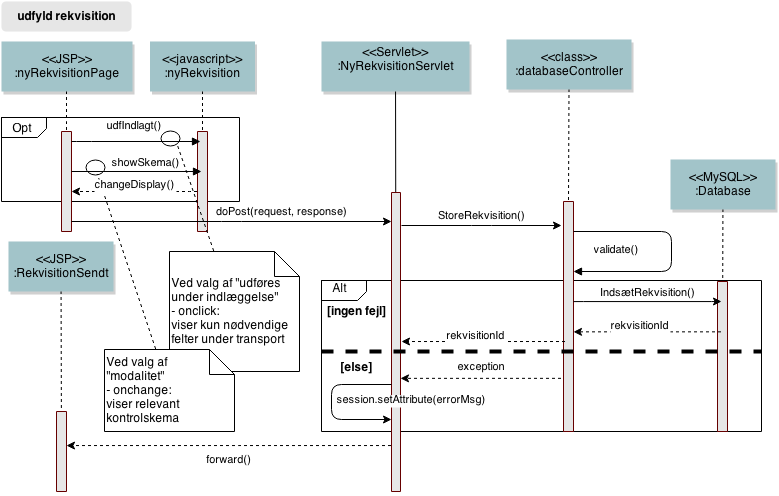
\includegraphics[width=\textwidth]{DSD}}
\caption{\emph{Design sekvens diagram}. For use casen 'bestil røntgen'. En
bruger udfylder og sender en rekvisition. Boksen markeret “Opt” viser to mulige
javascript kald siden kan kalde. \label{dsd}}
\end{figure}
\FloatBarrier
\begin{figure}[h]
\subsection*{Aktivitetsdiagram (Martin)}
\addcontentsline{toc}{subsection}{Aktivitetsdiagram}
\centering
\makebox[\textwidth]{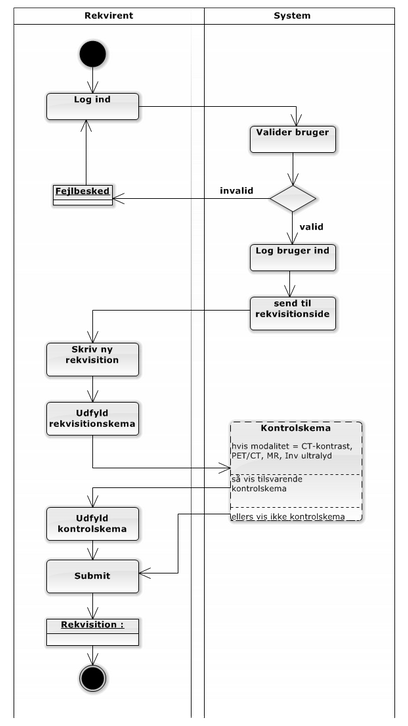
\includegraphics[width=\textwidth]{Aktivitetsdiagram}}
\caption{\emph{Aktivitetsdiagram for oprettelse og afsending af rekvisition}. I
diagrammet ses standard proceduren, når en rekvirent logger på systemet
og sender en rekvisition. Når han er logget ind, trykker han på ny rekvisition,
og alt efter hvilken modalitet rekvirenten vælger, bliver et kontrolskema
automatisk sat i forlængelse af rekvisitionen. \label{aktivitetsdiagram}}
\end{figure}
\FloatBarrier
\begin{figure}[h]
\subsection*{Data Flow diagram (Martin)}
\addcontentsline{toc}{subsection}{Data Flow diagram}
\centering
\makebox[\textwidth]{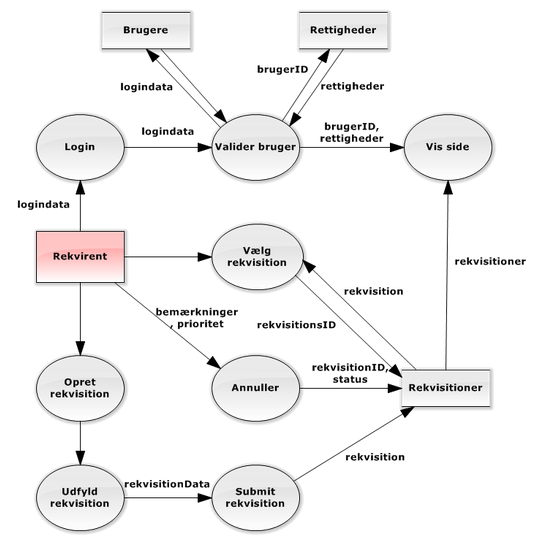
\includegraphics[width=\textwidth]{Data_Flow_diagram}}
\caption{\emph{Data Flow diagram}. Viser, hvordan data færdes når aktør eller
system foretager en handling. Den lakserøde firkant symboliserer aktøren,
cirklerne symboliserer handlinger, firkanterne med de åbne sider symboliserer
tabeller i databasen og pilene symboliserer data, der bliver sendt. For Data
Flow diagram af use casen visitér, se \hyperref[Bilag20]{bilag 20}.
\label{data_flow_diagram}}
\end{figure}
\FloatBarrier
\begin{figure}[h]
\subsection*{Database diagram (Rúni)}
\addcontentsline{toc}{subsection}{Database diagram}
\centering
\makebox[\textwidth]{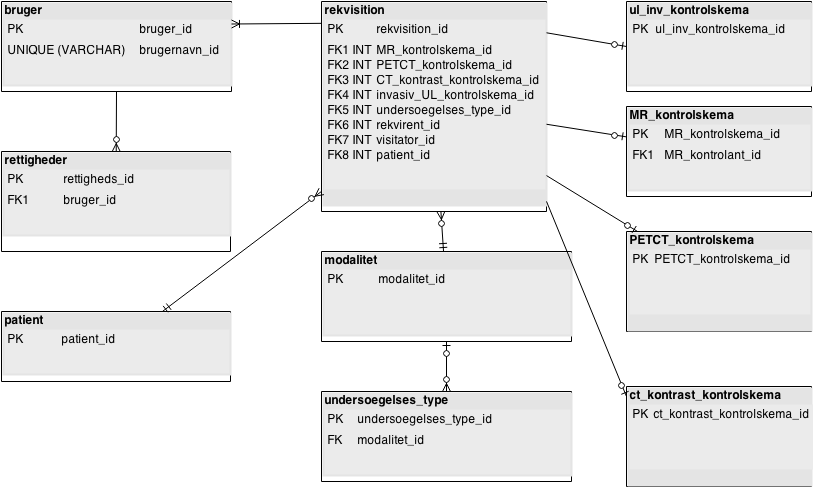
\includegraphics[width=\textwidth]{Database_diagram}}
\caption{\emph{Overordnet database diagram}. For at give et bedre overblik har
vi udeladt en del attributter der udelukkende indeholder data, disse kan ses i
det fulde database diagram i \hyperref[Bilag21]{bilag 21}.
\label{database_diagram}}
\end{figure}
\FloatBarrier
\subsubsection*{Mapning (Magnus)}
\addcontentsline{toc}{subsubsection}{Mapning}
I forhold til E/R diagrammet (se \hyperref[er_diagram]{figur
\ref*{er_diagram}}) har vi mappet vores brugere ved at tilknytte forskellige
rettigheder, alt efter deres funktion. Dette gør at vi fleksibelt kan give en
bruger flere rettigheder efter behov, og i tilfælde af udvidelser til softwaren
kan nye rettigheder simpelthen tilføjes til tabellen. Nedarvningen i
undersøgelses-typen er klaret ved at mappe alle data til en enkelt tabel.
Overlappende data fra de forskellige undersøgelses typer er mappet til tabellen
rekvisition, denne inkluderer også links til alle kontrolskemaerne, der
indeholder de resterende data der ikke overlapper, irellevante kontrolskemaer er
så sat til null. Vi har valgt denne fremgangsmåde da det var den simpleste for
os at implemetere, dog betyder det at hvis der i fremtiden tilføjes flere
undersøgelses modaliteter så skal disse også tilføjes til databasen.
\subsection*{Deployment (Christian)}
\addcontentsline{toc}{subsection}{Deployment}
Vi valgte at deploye vores system på to forskellige måder. Til udviklingsbrug
brugte vi en lokal Apache Tomcat server og DTU's MySQL database, da det var
hurtigt at afprøve ændringer og det kunne ske uden at påvirke vores fælles
kodebase.\\
Da vi også gerne ville have brugernes input, valgte vi desuden at deploye en
udgave på en cloud testserver. Vi oprettede et virtuelt serverinstance (kan
tilgås på \href{http://rtgrek-area51.rhcloud.com/}) på \href{www.openshift.com}.
Herpå kørte vi en Apache Tomcatserver og en mySQL server, således at
slutbrugerne kunne afprøve løsningen i dens aktuelle udformning.
FloatBarrier
\begin{figure}[h]
\centering
\makebox[\textwidth]{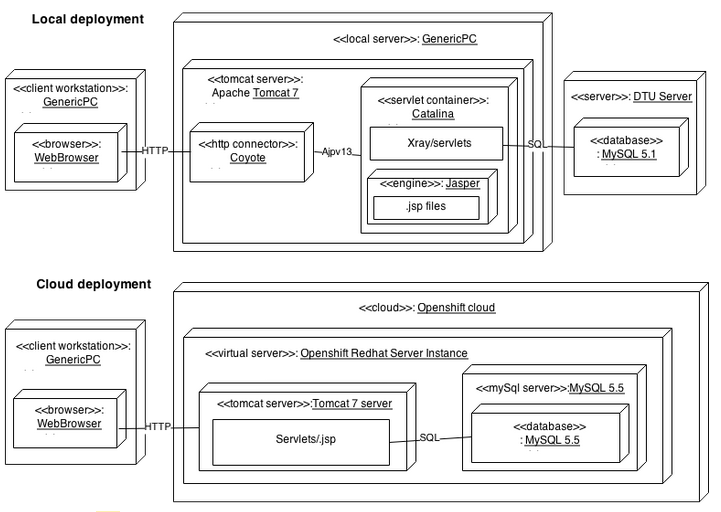
\includegraphics[width=\textwidth]{Deployment_diagram}}
\caption{\emph{Deployment diagram}. Vores lokale deployment kører på en Apache
Tomcat server. Serverens Coyote modul lytter efter http requests fra en browser
og videredelegerer Servlet og .jsp requests til Catalina servletcontaineren.
Containeren har en Jasper engine, der compiler .jsp siderne til servlets ved
deployment. Servlets kommunikerer med DTU's MySQL server. Vores Cloud deployment
kører tilsvarende på en Apache Tomcat server, der dog afvikles på en virtuel
Redhat server i Openshifts cloud. På den samme virtuelle server afvikles en
MySQL server. \label{deployment_diagram}}
\end{figure}
\FloatBarrier